\section{Полнотекстовый поиск}

\subsection{Введение}

Оговоримся заранее, что интересующие нас данные представлены в виде \textbf{документов}, каждый из которых имеет набор \textbf{полей}, некоторых свойств, значения которых принадлежат некоторому домену. Для удобства легче всего считать, что все поля~--- байтовые строки. Это представление удобно тем, что естественно для данных, представимых внутри компьютера и кроме того, лексикографический порядок байтовых массивов соответствует естественному порядку чисел, дат и лексикографическому порядку строк например в представлении UTF-16. Также удобно считать, что одному и тому же полю может соответствовать несколько значений. Пара (поле, значение) называется \textbf{термом} и обладает семантикой слова в тексте.

Любой документ можно привести к такой форме. Даты например при этом переводятся в числа, а числа в байтовые строки фиксированной длины, соответствующей размерности числа. Процесс приведения текста чуть более сложен и включает в себя две стадии~--- токенизирование, когда текст превращается в набор слов-токенов, каждый из которых затем анализируется, то есть приводится к нормальной форме. Для естественных языков это может быть например выделение корня из слова. Морфологический анализ слов является отдельной задачей, которая используется при построении полнотекстовых индексов, но которую мы не будем подробно затрагивать далее в тексте.

После того, как каждый документ приведен к форме набора термов, можно составить так называемые прямой и обратный индексы. Прямой индекс, который мы можем во многих формах наблюдать в реальности, отображает документ в виде какого-то уникального идентификатора, например абстрактного номера, в набор термов. Обратный индекс нужен для противоположной задачи, отобразить терм в набор документов, в которых он встречается. После того, как мы построили эти индексы, мы может обрабатывать запросы, включающие в себя термы, их отрицание и логические связки.

\begin{figure}[h]
	\centering
	\caption{Пример прямого и обратного индексов}
	
	\begin{subfigure}[b]{0.7\linewidth}
		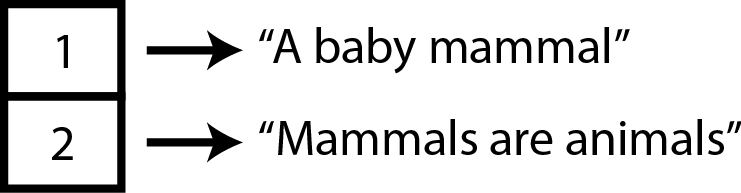
\includegraphics[width=\linewidth]{2-sample-index}
		\caption{Прямой индекс}
	\end{subfigure}
	
	\begin{subfigure}[b]{0.7\linewidth}
		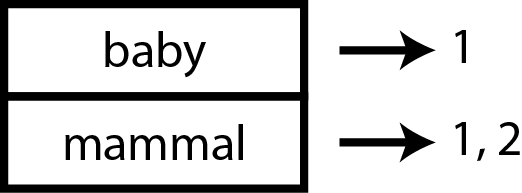
\includegraphics[width=\linewidth]{3-sample-reversed-index}
		\caption{Часть обратного индекса}
	\end{subfigure}
\end{figure}

Такой набор возможностей уже позволяет достаточно полно обрабатывать специальные и полнотекстовые запросы, то есть запросы, также сформулированные на естественном языке. С такими запросами необходимо проделать ту же процедуру, что и с исходными документами, преобразовав их к набору термов, затем по каждому терму получить множество документов, которые соответствуют терму, и после этого применить некоторые теоретико-множественные операции к получившимся наборам документов.

Отдельная задача состоит в ранжировании выборки, то есть сортировке формально подходящих документов по убыванию релевантности документа запросу. В данной области опять же существует множество подходов. Обычно все подходы сводятся к подсчету некоторой численной метрики для каждого документа, зависящей от параметров запроса и индекса. По этой метрике и производится сортировка. Примерами может служить метрика TF-IDF, берущая свое начало в работах Питера Луна\cite{luhn} и Карена Джоунса\cite{jones}, или PageRank\cite{google}, разработанная на заре поискового движка Google, особенная тем, что использует информацию, не связанную напрямую с содержанием текста.

Полнотекстовые запросы и запросы, вручную собранные из термов и логических связок не исчерпывают возможности поисковых систем. Также существуют нечеткие поисковые запросы, которые могут находить по похожим термам; поисковые запросы, сформулированные на языке регулярных выражений; поисковые запросы по фразе, когда порядок слов и то, что они идут в тексте последовательно, имеет значение. Каждый перечисленный вид поисковых запросов является по отдельности большой задачей достойной отдельного исследования.

Важным термином, связанным с полнотекстовым поиском, является так называемый Real Time поиск и Near Real Time (NRT) поиск. Данные термины связаны с тем, что если у нас есть непрерывный процесс генерации и соответственно индексации новых данных, то может быть задержка между тем, как мы проиндексировали документ в системе и тем, как мы теоретически можем его получить в составе поисковой выдачи. Это может быть связано с техническими особенностями построения индекса. Real Time поиск гарантирует, что такой задержки не существует и после того, как мы получили так или иначе подтверждение о том, что запрос на индексацию завершился успешно, документ гарантированно можно будет найти соответствующим поисковым запросом. NRT формально не определяется и предполагает, что задержка, хотя и существует, достаточно мала и незаметна с точки зрения пользователя. Свойство RT или NRT очень желательны в системе, так как обеспечивает незамедлительную обратную связь пользователю на его действия над данными в системе.

\subsection{Масштабируемость}

Иногда данных в системе настолько много, что они физически не вмещаются на одно устройство, или поток запросов становится настолько высок, что один сервер не справляется с такой нагрузкой, в этом случае применяют стратегии горизонтального масштабирования, а именно \textbf{шардинг} и \textbf{репликацию}.

Шардинг~--- разделение данных на непересекающиеся части, каждая из которых работает независимо, чаще всего независимо по вычислительным ресурсам. Каждый шард представляет собой отдельный индекс, к которому применяется запрос. Результатом применения запроса к шарду~--- некоторая выборка документов. После того, как запрос выполнился на каждом шарде, результаты объединяются в конечную выборку, которая и является ответом на запрос к шардированному индексу. Чаще всего объединение происходит по метрике релевантности, которая была рассмотрена выше, вследствие чего, при необходимости получения запроса размера $N$ при $K$ шардах, нельзя обойтись без того, чтобы не запросить $N$ наиболее релевантных документов с каждого шарда, так как мы не знаем, какие из них в итоге попадут в выборку. Это в $K$ раз увеличивает количество документов, которые будут извлечены из индекса, переданы по сети и агрегированы на сервере, обслуживающем клиентский запрос.

Таким образом, шардинг позволяет разделить индекс на части меньше размера, каждая из которых является подъемной для одного вычислительного узла. Это позволяет строить индексы колоссальных размеров. В свою очередь данный процесс отрицательно сказывается на производительности системы при обращении к ней пользователей.

Чтобы производить шардинг, каждый документ также должен обладать некоторым внешним по отношению к индексу параметром, в некоторых источниках упоминающимся как роутинг, по которому происходит выбор, в какой шард попадет этот документ. Роутинг не обязательно должен быть уникальным для каждого документа, но он должен обладать двумя важными свойствами. Во-первых, роутинг должен быть равномерно распределен по документам, так как иначе создается дизбаланс в нагрузке и в какой-то момент может получиться так, что при обработке запроса все шарды, кроме одного, самого большого, простаивают. Во-вторых, роутинг не должен меняться при изменении документа, так как иначе изменение может оказаться некорректным.

Репликация~--- копирование данных на независимые вычислительные мощности. Зачастую применяется в совокупности с шардированием, когда исходных индекс разбивается на несколько независимых частей, каждая из которых реплицируется. Репликация позволяет достигнуть двух важных вещей. Во-первых, используя ту или иную технологию распределения нагрузки между репликами, мы можем получить улучшения производительности системы, за счет того, что запросы к одному и тому же индексу исполняются на разных вычислительных мощностях. Это, например, может компенсировать проседание производительности при шардировании. Во-вторых, репликация данных позволяет обеспечить большую степень отказоустойчивости, об этом будет подробно рассказано ниже.

Однако, с увеличением производительности при поиске происходит уменьшение производительности при индексации, так как нам необходимо каждый раз записывать новые данные не в один индекс, а в каждую реплику, которых может быть 2 и более. Кроме того, наличие реплик может привести к проблемам, известным в области распределенных вычислений как stale reads, когда запросы на разные реплики дают разные результаты, так как запись прошла на одной реплике, но не прошла на другой. Об этом также будет сказано ниже.

\subsection{Отказоустойчивость}

В реальном мире компьютеры, на которых запускается программное обеспечение зачастую отказывает в силу тех или иных причин, по мере роста и масштабирования системы вероятность того, что в данный промежуток времени произойдет сбой, растет очень быстро, поэтому важно, чтобы система сохраняла работоспособность даже при условии, что произошел сбой, возможно даже не единственный.

Основная мера по предотвращению такой ситуации~--- создание распределенной системы без единой точки отказа, когда каждый функциональный узел дублируется на независимых вычислительных машинах. Таким образом, чтобы соответствовать стандартам качества и отказоустойчивости, необходимо, чтобы система, выполняющая поисковые запросы, была распределенной и умела реагировать на экстренные ситуации.

Если шард поискового индекса будет существовать в кластере в единственном экземпляре, то об отказоустойчивости не может идти речи. Выход из строя узла, на котором расположен шард приведет к невозможности обслуживания запросов к данному индексу. Таким образом, краеугольный камень работы поискового движка в условиях распределенности~--- репликация данных.

Из-за появления структуры данных, распределенной на несколько компьютеров в сети, возникает необходимость в гарантии консистентности системы в смысле корректности ее поведения с точки зрения внешнего наблюдателя. Как мы обсуждали ранее, для нашего применения система должна быть CP, то есть быть устойчива к разрывам связи в сети и обеспечивать линеаризуемость операций над данными.

\subsection{Существующие решения}

В предыдущих параграфах мы рассмотрели несколько задач, каждая из которых является предметом пристального изучения исследователей в области компьютерных наук, занимая все время на ее изучение и аккуратную реализацию. Кроме того, это не все задачи, связанные с создание собственной системы для построения полнотекстовых индексов. Среди тех, которые не были упомянуты ранее можно вспомнить алгоритмы сжатия и хранения данных для поиска или алгоритмы для построения и оптимизации поисковых запросов. Ввиду такой ситуации видится невозможным создавать собственное решение для полнотекстового поиска, так как это займет слишком большой объем времени и сил при итоговых результатах, несопоставимых с уже существующими.

Вследствие таких рассуждений было решено для задачи построения индексов и осуществления полнотекстового поиска использовать готовые инструменты. Крайне желательным качеством готового программного обеспечение является его открытость. Это позволяет лучше понимать устройство системы, в первую очередь для оперативного решения возникающих проблем. Таким образом, выбор пал на уже реализованные, зарекомендовавшие себя ранее движки для полнотекстового поиска с открытым исходным кодом. В результате анализа существующих аналогов, были выбраны и рассмотрены следующие альтернативы.

Apache Lucene\cite{lucene} реализовывает функционал по работе с полнотекстовыми индексами, но не предоставляет интерфейса для внешних сервисов и встроенных возможностей по созданию распределенной системы.

Sphinx, кроме реализации полнотекстовых индексов и работы с ними, предоставляет также внешний интерфейс для приложений, которые будут использовать этот движок. Однако работа по распределению индексов на несколько компьютеров не автоматизирована, хоть инструменты для этого и есть.

Последние два решения, Apache Solr и Elasticsearch, очень похожи между собой. Оба предоставляют богатый внешний интерфейс для конечного приложения. Оба автоматически управляют распределенными индексами и предоставляют инструменты для горизонтального масштабирования.

Рассмотрим каждое решение подробно.

\subsubsection{Apache Lucene}

Lucene~--- фреймворк, созданный на платформе Java, для создания индексов для полнотекстового поиска и последующего поиска информации в них. Данный фреймворк решает задачи, связанные с построением индексов как структур данных в памяти и на постоянном носителе; предварительным анализом текста и приведением его к нормальной форме, упомянутой выше, необходимой для организации поиска; выполнением поисковых запросов, в том числе переписывание их для лучшей производительности и релевантности и многие другие.

Однако сконцентрировавшись на задачах полнотекстового поиска, данный фреймворк не предусматривает создание распределенной системы хранения индексной информации исключительно с помощью средств самого фреймворка. Используя данное решение, задачи горизонтального масштабирования, предоставления интерфейса внешнему пользователю и индексирования данных в контексте данного проекта должны быть решены программистом самостоятельно.

Несмотря на то, что многие задачи оказываются покрыты функциональностью данного решения, не меньшее количество задач остается нерешенными. Среди них одни из самых сложных, связанные с надежностью и консистентностью поисковых индексов. По данным причинам было решено отказаться от Lucene в чистом виде.

\subsubsection{Sphinx}

Sphinx~--- готовая платформа для полнотекстового поиска, написанна на C++, используя в своей основе существующие базы данных и обладающая SQL-синтаксисом запросов, что очень удобно для встраивания в процессы, уже использующие подобный синтаксис для осуществления запросов к массивам данных. Данное решение обладает за счет своей архитектуры высокой производительностью как при индексации документов, так и при поиске. Для приложения, где производительность важнее всего, Sphinx среди всех остальных решений подойдет больше всего.

Однако как решение существующей задачи Sphinx подходил плохо, так как обладал скудным функционалом для создания распределенных индексов, требуя при этом большое количество ручной работы, от чего изначально хотелось избавится.

\subsubsection{Elasticsearch}

Elasticsearch~--- тоже готовая платформа, основанная на Lucene. Данное решение, полагаясь на качество построения индексов и поиска по ним, обеспечивающееся уже существующей библиотекой, концентрируется на обеспечении распределенной системы с готовым сетевым интерфейсом, решающее такие задачи, как репликация данных, поддержка синхронизации данных между репликами, обработка разделений сети и так далее.

Elasticsearch поддерживает дополнительные уровни абстракции, необходимые для оперирования большими объемами данных на множестве вычислительных узлов, и выполняет операции, необходимые для поддержки подобных абстракций и операций над ними. Например, ключевым понятием в данной системе является индекс, который состоит из некоторого количества шардов. Каждая реплика шарда назначается на некоторый узел в кластере Elasticsearch, после чего средствами Lucene на этом узле создается уже физический индекс. В этом индексе в дальнейшем содержатся документы, и в нем же происходит поиск.

По архитектуре Elasticsearch представляет собой систему с единым мастером, который выбирается с помощью протокола распределенного консенсуса Zen, реализованного специально для данного решения. После того, как мастер был выбран, только он может производить мутации состояния, такие как создание новых и удаление старых индексов, назначение шардов на узлы, добавление узлов в кластер и исключение узлов из кластера и так далее. Если мастер еще не выбран, то по-умолчанию допускаются запросы на чтение, но не на запись, что, впрочем, можно изменить с помощью конфигурации. В случае возникновения разделения в сети, мастер не выбирается, если только в текущей доле не находится достаточно оперирующих узлов, которые могут стать мастером.

Очень важно особенностью Elasticsearch является богатый специальный язык для написания запросов к индексам, поддерживающий вкладывающиеся запросы, логические связки и множество типов самих запросов, дублирующих и дополняющих функциональность Lucene. Также, кроме основной способности находить набор наиболее релевантных документов среди всех, добавленных в индекс, Elasticsearch отличается большим набором функций для агрегации данных и нахождение различных метрик и статистики по данным, что открывает богатые возможности по анализу данных и подготовке отчетов по большим объемам информации.

Покрывая множество задач, связанных с полнотекстовым поиском в распределенной системе, Elasticsearch имеет некоторое количество недостатков, как то недостаточная надежность, сырость протокола распределенной синхронизации, отсутствие API для управления задачами и так далее. Однако положительные стороны в достаточной мере оправдывают меры предосторожности, необходимость в грамотной эксплуатации и тщательном мониторинге системы, чтобы потенциально выбрать данное решение.

\subsubsection{Apache Solr}

Во многом схоже с Elasticsearch, Solr является распределенной системой, которая в своей основе для полнотекстового поиска использует библиотеку Lucene. Главным отличием от конкурента в положительную сторону заключается в протоколе синхронизации, который используется в Solr. В выборе мастера Solr полагается на другой продукт от Apache Foundation, Zookeeper, который исключительно фокусируется на создании системы для распределенных блокировок, за счет чего имеет большую степень надежности в случаях неполадок и возникновения разделения сети.

В остальном архитектура Solr очень похожа внешне на архитектуру Elasticsearch, за исключением может быть не такого гибкого и развитого языка запросов и агрегаций. Однако, тогда как Elasticsearch поставляет внешний интерфейс поверх HTTP+Json, в Solr этим не ограничивается и транспорт гораздо более разнообразен, что позволяет встроиться в большинство существующих систем.

\subsection{Выбор решения}

В силу факторов, указанных выше, Sphinx и чистый Lucene не рассматривались, как возможные варианты при реализации финальной системы. Вследствие этого выбор сузился до одного из двух вариантов, очень похожих между собой, Solr или Elasticsearch. Для того, чтобы сделать осмысленный вывод, был произведен анализ различных аспектов этих двух решений, включающий такие вопросы, как производительность поиска и индексации, язык запросов, его удобство в использовании и совместимость с существующими системами, требование к содержанию и поддержке и так далее.

В результате анализа было принято решение использовать Elasticsearch, так как его возможности и удобство использования и эксплуатации перекрывали преимущества конкурента\cite{solr-vs-es-features}. Кроме того, чаще всего в приложениях одновременно с поиском осуществляется активная индексация новых данных, а в подобных условиях известно, что Solr проигрывает по производительности поиска и индексации\cite{solr-vs-es-perf-1}, когда как в обратной ситуации Solr был бы предпочтительным выбором по параметру быстродействия\cite{solr-vs-es-perf-2}.

\clearpage
